\chapter{Natural language}
\label{ch:natural-language}
\begin{flushright}
\emph{The fish trap exists because of the fish; once you've gotten the fish,\\
you can forget the trap. The rabbit snare exists because of the rabbit;\\
once you've gotten the rabbit, you can forget the snare.\\
Language exists because of meaning; once you've gotten the meaning,\\
you can forget language.}\\ --- Zhuangzi (4th Century BC)
\end{flushright}
\minitoc

\section{Natural language is not essential to AGI}

Our approach is to define a logic that can faithfully render arbitrary natural-language texts.  We call such a logical form Geniform.  The translation of NL to Geniform can itself be encoded as logical rules, thus the parsing of NL can be achieved via logical inference (as forward-chaining in a bottom-up manner).  And since logical inference is reversible, the generation of NL will also come as free.

All the irregularities of NL will be taken care of via machine learning.

\subsection{Background: unification-based grammars}

The family of unification-based grammars includes LFG (Lexical Functional Grammar), HPSG (Head-Driven Phrase Structure Grammar), and PATR grammar.  The unification algorithm used in unification-based grammar is the same as the unification algorithm used in logic.  This is further evidence that the brain employs abstract symbolic processing similar to formal logic.

\subsection{Background: cognitive linguistics}

Our approach is closer to ``formal semantics''.  Many authors, most famously Richard Montague, have argued that natural languages are formal languages.  Some have also advocated the use of natural language as knowledge representation in AI.  Thus the line between formal and natural languages is blurred.

\todo{How may cognitive linguistics affect natural language processing in Genifer?}

\section{Abduction as interpretation}
\label{sec:abduction-as-interpretation}

\subsection{A detailed example}

The general sequence is:\\
\hspace*{1cm} tokenization $\rightarrow$ POS-tagging $\rightarrow$ syntax parsing $\rightarrow$ semantic parsing\\
which should be familiar to everyone with experience in NL processing.

I will explain the details using a simple example:\\
\hspace*{1cm} ``I love Mary''

The crucial thing is that we represent everything in a logic-based framework. First we represent the sentence as "raw data" (ignoring tenses to simplify matters):\\
\hspace*{1cm} $\mbox{sentence}(e_0)$\\
\hspace*{1cm} $\mbox{lexeme-I}(e_1)$\\
\hspace*{1cm} $\mbox{lexeme-love}(e_2)$\\
\hspace*{1cm} $\mbox{lexeme-Mary}(e_3)$\\
\hspace*{1cm} $\mbox{begins-with}(e_0, e_1)$\\
\hspace*{1cm} $\mbox{follows}(e_2, e_1)$\\
\hspace*{1cm} $\mbox{follows}(e_3, e_2)$\\
where:\\
\hspace*{1cm} the $e_i$'s are \textbf{entities} (logical constants).\\
\hspace*{1cm} the entities $e_1$, $e_2$, and $e_3$ are words.\\
\hspace*{1cm} follows() means a word follows another word in a sentence.

Up to now, all we have is a sentence as raw text (without meanings).  The next step is to recognize parts of speech (nouns, verbs, adjectives, etc). We can use logical rules to do this.

An example logical rule is:\\
\hspace*{1cm} $\mbox{lexeme-Mary}(X) \rightarrow \exists e \; \mbox{parse-as}(e, X) \wedge \mbox{noun}(e)$\\
which simply means that the word "Mary" is a noun. X is a variable (implicitly universally quantified). $e$ is a new entity, which instantiates to $e_4$ when the rule is applied.

We can also use logical rules to parse syntax. We can perform ``VP $\leftarrow verb + noun$'' with this rule\footnote{We need this special rule:\\
\hspace*{1cm} $\mbox{follows}(X_1, X_2) \wedge \mbox{parse-as}(X_1, X_3) \wedge \mbox{parse-as}(X_2, X_4) \rightarrow \mbox{follows2}(X_3, X_4)$ }:\\
\hspace*{1cm} $\mbox{verb}(X_1) \wedge \mbox{noun}(X_2) \wedge \mbox{follows2}(X_2, X_1) \rightarrow \exists e \; \mbox{parse-as}(e, X_1, X_2) \wedge vp(e)$\\
which creates a new entity $e_5$ which is a VP.

Assume that eventually we have a parse of the sentence S, $e_6$. Notice that up to now, it's all syntax parsing.

Next we perform semantic parsing.  The key is to generate partial meanings for phrases, such as the verb phrase ``loves Mary''.

\textbf{Lambda operator.}  In formal semantics, it is customary to use the $\lambda$ operator to represent the meaning of phrases.  The reason is that first-order logic do not have the expressive power to represent such phrases.  For example, the VP ``loves Mary'' denotes ``somebody's loving Mary'', which may be represented as $love(\_ \,,mary)$; but that is not a well-formed formula in FOL.  Instead we can represent it using the $\lambda$ expression $\lambda x \; love(x,mary)$.

\textbf{Composition of concepts.}  (For details see \S\ref{sec:composition})  Under this method, all phrases are represented by compositions.  For example, the VP ``loves Mary'' can be represented by $app(loves,mary)$, or in short form $mary \circ loves$.  This composite is a \textit{first-order object}, ie, a first-class citizen in the logic which can be further manipulated or modified, eg, when we compose it with $john$, we get $((mary \circ loves) \circ john)$ which is equivalent to the FOL statement $loves(john,mary)$.

I think this method is superior to $\lambda$ because the meanings of phrases can be represented by first-order objects.  It also makes semantic parsing very intuitive.

% \todo{Revise this example with the newly improved Geniform.}

\todo{Explain semantic parsing with examples.}

%A semantic rule is similar to a syntactic one:\\
%\hspace*{1cm} $\mbox{lexeme-love}(X) rightarrow \exists e \; \mbox{parse-as}(e, X) \wedge \mbox{verb}(e) \wedge \mbox{means}(e, \mbox{concept-love})$\\
%
%\hspace*{1cm} $\mbox{verb}(X_1) \wedge \mbox{np}(X_2) \wedge \mbox{follows2}(X_2, X_1) \wedge \mbox{means}(X_1, Y_1) \wedge \mbox{means}(X_2, Y_2)$\\
%\hspace*{1cm} $rightarrow \exists e \; \mbox{parse-as}(e, X_1, X_2) \wedge vp(e) \wedge \mbox{means}(e, comp(Y_1,Y_2))$\\
%
%For example, we can augment the syntactic rule\\
%\hspace*{1cm} $\mbox{VP} \leftarrow \mbox{verb}, \mbox{NP} $\\
%with\\
%\hspace*{1cm} $\mbox{VP}(\mbox{comp}(Sem_1,Sem_2)) \leftarrow \mbox{verb}(Sem_1), \mbox{NP}(Sem_2)$\\
%where the $Sem$'s are variables containing the ``semantics'' of phrases.\\
%\hspace*{1cm} $\mbox{S} \leftarrow \mbox{NP}, \mbox{VP} $\\
%\hspace*{1cm} $\mbox{S}(Predicate) \leftarrow \mbox{NP}(Subject), \mbox{VP}(Subject * Predicate) $\\
%\hspace*{1cm} $\mbox{VP}(X) rightarrow \mbox{com}(\mbox{loves},\mbox{mary})$\\
%which creates a new entity $e_7$ with the meaning of "love".\\
%\hspace*{1cm} $\mbox{lexeme-love}(X_1) rightarrow \exists e \; \mbox{concept}(e) \wedge \mbox{means}(e, \mbox{concept-love})$\\
%
%The final step of semantic parsing uses a special trick,  ``de-reification'' (\S\ref{sec:reification}):\\
%\hspace*{1cm} (assume that $e_{8}, e_{9}$ denote the persons John and Mary)\\
%\hspace*{1cm} $\mbox{de-reify}(\mbox{concept-love}, e_{8}, e_{9})$\\
%which generates the logical statement:\\
%\hspace*{1cm} $\mbox{loves}_1(e_{8},e_{9})$\\
%
%Finally we have:\\
%\hspace*{1cm} $\mbox{means}(e_0, \mbox{loves}_1)$

\section{Comprehensive grammatical categories of English}

Here are some NL grammatical categories (intended to cover as broadly as possible) and typical examples in English.  Designers of NL interfaces can supply translations to these examples.  [The contents in this section and all the examples are taken directly from the book "English Grammar" by Peter Collins, 1998, Addison Wesley.  \todo{NOTE:  This may be a copyright infringement but I have contacted the author without getting his reply.}]  This page is intended to provide a simple comparison of NL interfaces, not meant to be a standard grammar for AGI purposes.

\titleformat{\subsection}[hang]{\sffamily\bfseries\large\color{blue}}{(\Alph{subsection}) \hspace{5pt}}{0pt}{}

\setcounter{subsubsection}{1}
\renewcommand{\subsubsection}[1]{\sffamily{\bfseries{\color{blue}{ \stepcounter{subsubsection} (\Alph{subsection}.\arabic{subsubsection}) \hspace{5pt}#1}}}}

\newcounter{subsubsubsection}[subsubsection]
\newcommand{\subsubsubsection}[1]{\stepcounter{subsubsubsection} \sffamily{\bfseries{\color{blue}{ (\Alph{subsection}.\arabic{subsubsection}.\arabic{subsubsubsection}) \hspace{5pt}#1}}}}

\subsection{Nouns}

\subsubsection{Common nouns}

eg \english{chair}, \english{chairs}

eg \english{importance}

\subsubsection{Proper nouns}

eg \english{Australia}

eg \english{The Isle of Man}

\subsubsection{Pronouns}

eg \english{he}

eg \english{\textbf{our} chair} (possessive, as determiner)

eg \english{theirs}

eg \english{each other}, \english{one another} (reciprocal pronouns)

eg \english{this}, \english{that} (demonstrative pronouns)

eg \english{who}, \english{whom}, \english{whatever} (interrogative and relative pronouns)

eg \english{some}, \english{both}, \english{any}, \english{each}, \english{none}, \english{nobody} (indefinite pronouns)

\subsection{Verbs}

\subsubsection{Main verbs}

eg \english{kick}, \english{grow}

eg \english{to kick}, \english{kicked}, \english{kicking}, \english{kicks} (tenses and other inflections)

\subsubsection{Auxiliary verbs}

eg \english{can}, \english{have}, \english{haven't}

eg \english{She \textbf{is} dancing the lambada.}

eg \english{He \textbf{has} driven for 4 hours.}

\subsubsection{Operators}

eg \english{they \textbf{will} try their best}, \english{Sam \textbf{won't} play chess}

\subsection{Adjectives}

\subsubsection{Attributive (modifies a head noun)}

eg \english{the \textbf{loud} bell}

\subsubsection{Predicative}

eg \english{the bell was \textbf{loud}}

\subsubsection{Gradation}

eg \english{\textbf{very} loud}, \english{\textbf{a bit} loud}

\subsubsection{Comparison}

eg \english{louder}, \english{loudest}

\subsection{Adverbs}

eg \english{The policeman acted \textbf{decisively}}

eg \english{He is a \textbf{somewhat} shy young man}

eg \english{\textbf{Actually}, many of the lifeboats have been removed}

eg \english{Patrick has lost 2 games, \textbf{however} he could still win}

eg \english{more surprisingly}, \english{most surprisingly}

\subsection{Determinatives}

\subsubsection{Articles}

eg \english{the}, \english{a}, \english{an}

\subsubsection{Demonstratives}

eg \english{this}, \english{that}, \english{those}

\subsubsection{Interrogatives}

eg \english{which}, \english{what}

\subsubsection{Cardinal numerals}

eg \english{one}, \english{two}

\subsubsection{Quantifiers}

eg \english{both}, \english{all}, \english{every}, \english{any}, \english{no}, \english{much}, \english{less}

\subsubsection{Prepositions}

\subsubsubsection{Time}


eg \english{\textbf{after} our match}, \english{\textbf{during} the exam}

\subsubsubsection{Place}


eg \english{\textbf{in} the kitchen}, \english{\textbf{against} the wall}

\subsubsubsection{Manner}


eg \english{\textbf{with} ease}

\subsubsubsection{Agency}


eg \english{\textbf{by} the mechanic}

\subsubsubsection{Recipience}


eg \english{\textbf{to} a friend}

\subsubsection{Subordinates}

\subsubsubsection{Time}


eg \english{\textbf{until} it rains}, \english{\textbf{as} she spoke}

\subsubsubsection{Condition}


eg \english{\textbf{if} we win Lotto}, \english{\textbf{unless} a catastrophe occurs}

\subsubsubsection{Concession}


eg \english{\textbf{although} she likes coffee}, \english{\textbf{while} it was undoubtedly entertaining}

\subsubsubsection{Contrast}


eg \english{\textbf{whereas} Japan is a creditor nation}

\subsubsubsection{Exception}


eg \english{\textbf{except} he didn't have the strength}

\subsubsubsection{Reason}


eg \english{\textbf{because} the bus broke down}

\subsubsubsection{Comparison}


eg \english{you ate more peanuts \textbf{than} I did}

\subsubsection{Coordinators}

eg \english{Peter went to Paris \textbf{but} his family stayed home}

eg \english{Barbie was wearing a new bracelet \textbf{and} a diamond ring}

eg \english{Should we come before \textbf{or} after lunch?}

eg \english{\textbf{Both} Bill \textbf{and} his wife deny the allegations}

eg \english{She \textbf{neither} hates him \textbf{nor} loves him}

eg \english{It's \textbf{not} for you \textbf{but} for me}

\subsection{Phrases}

\subsubsection{Noun phrase (NP)}

eg \english{large birds with sharp claws}

eg \english{writers of science fiction, who are here for a conference}

\subsubsection{Verb phrase (VP)}

eg \english{[Lisa] \textbf{trains} 3 times a week}

eg \english{There I \textbf{am}, minding my own business, when this tall blonde \textbf{walks} up and \textbf{asks} me for a cigarette}

eg \english{Ken said, 'I \textbf{have} enough money' }

eg \english{[If I] \textbf{could} have my life over again, [I] \textbf{would} not change anything}

eg \english{[They should] \textbf{have reached} the peak by now}

eg \english{[Ken] \textbf{is} building a new house}

eg \english{[Many footballers] \textbf{get} injured}

\subsubsection{Adjective phrase (AdjP)}

eg \english{too rebellious}, \english{quite surprisingly intelligent}, \english{very slow}

eg \english{slower than a wet week}, \english{large for a goldfish}

eg \english{fiercer than I expected}

eg \english{sorry that he hurt her feelings} (noun clause)

eg \english{aware of the consequences} (of-PP)

\subsubsection{Adverb phrase (AdvP)}

eg \english{very quickly}, \english{most reluctantly}

eg \english{more defiantly than they had predicted}

\subsubsection{Prepositional phrase (PP)}

eg \english{\textbf{in} the water}

eg \english{\textbf{with} a spoon}

eg \english{[way] \textbf{below} standard}, \english{[just] \textbf{before} the start}

eg \english{Scott arrived \textit{in} \textbf{a limousine} \textit{with} \textbf{his girlfriend}}

\subsubsection{Genitive phrase (GP)}

eg \english{\textit{The princess's} popularity was greater than \textit{her husband's}}

\subsection{Clauses}

\subsubsection{Object vs predicative complements}

eg \english{Mary contacted \textbf{a police officer}} (object)

eg \english{Mary was \textbf{a police officer}} (predicative, \english{was}=copula)

\subsubsection{Subjective and objective predicatives}

eg \english{Indira was \textbf{generous}} (subjective)

eg \english{We considered Indira \textbf{generous}} (objective)

\subsubsection{Patterns of complementation}

\subsubsubsection{intransive (S P)}

eg \english{Sue \textbf{stumbled}}

\subsubsubsection{monotransitive (S P Od)}

eg \english{Sue \textbf{sipped a martini}}

\subsubsubsection{Copulative (S P PCs)}

eg \english{Sue \textbf{seems drunk}}

\subsubsubsection{Ditransitive (S P Oi Od)}

eg \english{Sue \textbf{offered her guests a martini}}

\subsubsubsection{Complex-transitive (S P Od PCo)}

eg \english{Sue \textbf{made them drunk}}

\subsubsection{Other complements}

\subsubsubsection{PP-complements of prepositional verbs}

eg \english{They have decided \textbf{on a short vacation}}

eg \english{He approves entirely \textbf{of your decision}}

eg \english{Geoff protected his little brother \textbf{from the bullies}}

eg \english{She blames all their problems \textbf{on his incompetence}}

\subsubsubsection{Adverbs as complement of phrasal verbs}

eg \english{Vera cried \textbf{out}}

eg \english{We give \textbf{up}}

eg \english{The umpires have called \textbf{off} the match}

eg \english{Please take the garbage \textbf{out}}

eg \english{We have come \textbf{up} \textbf{with an alternative plan}}

\subsubsubsection{Non-finite complements of 'catenative' verbs}

eg \english{I \textbf{plan} to \textbf{keep} applying for jobs}

eg \english{You should \textbf{stop} \textbf{trying} to \textbf{get} invited}

\subsubsection{Adjuncts}

AdvP: eg \english{very carefully}, \english{sometimes}, \english{moreover}

PP: eg \english{over the road}, \english{with a torch}

Subordinate clause:  eg \english{because it is raining}, \english{after the music stopped}

NP: eg \english{next Easter}, \english{this Friday}

types:

Time:  eg \english{at Easter}, \english{in 2 week's time}

Frequency:  eg \english{each Friday}, \english{on the hour}

Place: eg \english{in Bandung}, \english{on the summit}

Purpose: eg \english{in order to test the hypothesis}, \english{for a break}

Reason: eg \english{because he is shy}, \english{on the grounds of sanity}

Condition: eg \english{if you agree}, \english{unless it is convenient}

Manner: eg \english{more politely}, \english{with a spade}

Degree: eg \english{in my opinion}, \english{to be fair}, \english{unfortunately}

Connective: eg \english{consequently}, \english{in other words}, \english{however}

\subsubsection{Mood}

\subsubsubsection{Declarative mood}

eg \english{He is serious}

\subsubsubsection{Interrogative mood}

eg \english{Is he serious?}

eg \english{Anastasia has sent another e-mail, hasn't she?}

eg \english{Whose T-shirt is that?}

eg \english{Who can help me?}

eg \english{Where are my keys?}

\subsubsubsection{Imperative mood}

eg \english{Be serious}

eg \english{Give me some more money}

eg \english{Don't forget to write}

eg \english{Let's apply for a loan}

\subsubsubsection{Exclamative mood}

eg \english{How serious he is!}

eg \english{How many times have I asked you!}

\subsubsection{Negation}

clausal negation:  eg \english{Courtney is \textbf{not} reading}\\
                   eg \english{We have heard \textbf{nothing}}\\
                   eg \english{\textbf{Nobody} likes a loser}\\
                   eg \english{We \textbf{barely} made it}\\
                   eg \english{They \textbf{seldom} celebrate birthdays}

sub-clausal negation:  eg \english{Karen is very \textbf{unfriendly}}\\
                      eg \english{The ambulance arrived \textbf{not long ago}}

\subsection{Subordination and coordination}

\subsubsection{Subordinative clause (complex sentence)}

eg \english{I know \textbf{that Ella lives in Sydney}}

eg \english{He knows a woman \textbf{who lives in Sydney}}

eg \english{He asked \textbf{whether anyone had submitted a nomination}}

\subsubsubsection{Adverbial clauses}

time:  eg \english{Angelica will not agree to it \textbf{until his attitude improves}}

place:  eg \english{he goes \textbf{wherever his fancy takes him}}

etc

\subsubsubsection{Relative clauses}

eg \english{Is that the boy who you were referring to?}

eg \english{I remember the days when none of us had a care in the world}

eg \english{I know who is replacing you}

eg \english{Whatever is now developing can only cause harm}

\subsubsubsection{Comparative clauses}

eg \english{He performed worse than you did}

eg \english{Tim has won a larger grant than I have}

eg \english{She is as tall as we had anticipated}

\subsubsubsection{Non-finite clauses}

infinitival: eg \english{Sharon wants to \textbf{apply next year}}

present-participle: eg \english{Sharon favors \textbf{applying next year}}

past-participle: eg \english{Sharon has her application \textbf{lodged already}}

past-participle: eg \english{Anyone \textbf{caught smoking here} can be prosecuted}

\subsubsubsection{Verbless clauses}

eg \english{\textbf{If in doubt} consult your solicitor}

eg \english{He visits his parents \textbf{whenever possible}}

eg \english{\textbf{With Claudia in charge} we should be able to regain control}

\subsubsection{Coordinated clause (compound sentence)}

eg \english{Ella lives in Sydney, but she was born in China}

eg \english{Daphne like classical music \textbf{but} her husband prefers jazz}

\subsection{Information packaging}

\subsubsection{Topic}

eg \english{Leonardo da Vinci painted the Mona Lisa}\\
vs \english{The Mona Lisa was painted by Leonardo da Vinci}

\subsubsection{Focus}

eg \english{The judges gave near maximum points to Lipinsky}\\
vs \english{The judges gave Lipinsky near maximum points}

\subsubsection{Weight (more weight near end of sentence)}

eg \english{It surprised us that an Australian skier could win a medal in the slalom event at the Nagano Olympics}\\
vs \english{That an Australian skier could win a medal in the slalom event at the 
Nagano Olympics surprised us}

\subsubsection{Voice}

active: eg \english{Sergeant Rogerson arrested the thief}\\
passive: eg \english{The thief was arrested by Sergeant Rogerson}

eg \english{Each specimen was carefully dissected}

\subsubsection{Cleft sentences}

eg\\
\english{Whitlam recalled the remaining troops from vietnam}\\
\english{It was Whitlam who recalled the remaining troops from Vietnam}\\
\english{It was the remaining troops that Whitlam recalled from vietnam}\\
\english{It was from Vietnam that Whitlam recalled the remaining troops}

eg\\
\english{Salt air can cause rust}\\
\english{What can cause rust is salt air}\\
\english{Salt air is what can cause rust}

\subsubsection{Extraposition}

eg \english{It is a pity that CDs are so expensive}

\subsubsection{Existential sentences}

eg \english{There is a fly in my soup}

eg \english{There's been another oil spill}

eg \english{There's a present for you}

eg \english{There followed a new round of toasts}

\subsubsection{Reordering}

\subsubsubsection{Subject-complement reversal}

eg \english{Tom is the short one}\\
$\Longrightarrow$ \english{The short one is Tom}

\subsubsubsection{Topicalization}

eg \english{He rejects totally the corruption charge}\\
$\Longrightarrow$ \english{The corruption charge he rejects totally}

eg \english{It rained for most of the day last Saturday}\\
$\Longrightarrow$ \english{Last Saturday it rained for most of the day}

\subsubsubsection{Locative inversion}

eg \english{Another F15 appeared from behind the clouds}\\
$\Longrightarrow$ \english{From behind the clouds appeared another F15}

\subsubsubsection{Dislocation}

eg \english{Dr Davidson's never available on Wednesdays}\\
$\Longrightarrow$ \english{(As for) Dr Davidson, he's never available on Wednesdays}

\subsubsubsection{Dative movement}

eg \english{Steve gave a red rose to his girlfriend}\\
$\Longrightarrow$ \english{Steve gave his girlfriend a red rose}

\subsubsubsection{Extraposition from NP}

eg \english{A position for someone with programming expertise is available}\\
$\Longrightarrow$ \english{A position is available for someone with programming expertise}

\subsubsection{Some grammatical devices}

\subsubsubsection{Co-reference}

eg \english{Your sister rang yesterday. \textbf{She} asked if you could call her back.}

eg \english{It is inadvisable to visit Jakarta at present.  Civil unrest has broken out \textbf{there}.}

\subsubsubsection{Ellipsis}

eg \english{Come whenever you can [come]}

eg \english{Somebody should help dad.  I'll ask Barry to [help dad].}

\subsubsubsection{Substitution}

eg \english{I have 2 spare tickets for the concert.  Would you like \textbf{one}?}

eg \english{She achieved less this year than she \textbf{did} last year.}

eg \english{I'll collect the kids after school if you don't get the opportunity to \textbf{do so}.}

\titleformat{\subsection}[hang]{\sffamily\bfseries\large\color{blue}}{\thesubsection \hspace{5pt}}{0pt}{}

\renewcommand{\subsubsection}[1]{\sffamily{\bfseries{\color{blue}{ \stepcounter{subsubsection} #1}}}}

\section{Geniform -- a logical form for natural language}
\label{sec:geniform}

% Rus proposed a popular logical form for rendering natural language, which is of reference value.  Geniform has made several significant improvements over it.

The Geniform logical form is special in that it can represent all natural-language grammatical categories elegantly.  To illustrate this, consider:\\
\tab \english{John loves Mary}\\
which is rendered in predicate logic as:\\
\tab \formula{loves(john, mary)}\\
(ignoring tense).  But what if we want to say:\\
\tab \english{\textit{Loving Mary} is foolish} ?\\
The verb phrase \english{loving Mary} is a grammatical unit that has a specific meaning but it cannot be represented in predicate logic.  In computational linguistics we usually use the \textbf{$\lambda$-abstraction} to represent it:\\
\tab \formula{$\lambda$x.loves(x, mary)}\\
but as you can see, this form is not very human-readable.

% One idea is to replace $\lambda$-abstractions with \textbf{combinators}\footnote{This idea came from Curry's combinatory logic, which has computational power equivalent to that of $\lambda$-calculus.  The technique of Currying was also invented by Curry.}.  For example,\\
% \tab \formula{loves(x, y)}\\
% can be represented in \textbf{Curried form} as:\\
% \tab \formula{\textbf{loves} = $\lambda$y($\lambda$x.loves(x,y))}\\
% so that \formula{\textbf{loves}} is equivalent to the original predicate but it takes its arguments one at a time.

% Now we can represent elements like:\\
% \tab \english{John loves ....} as \formula{(\textbf{loves} john)} and\\
% \tab \english{.... loves Mary} as \formula{(\textbf{C loves} mary)}\\
% where \formula{\textbf{C}} is a combinator with the property \formula{\textbf{C}XYZ = \textbf{C}XZY}.

Instead of $\lambda$-expressions, Geniform uses \textbf{combinators} to represent concepts, resulting in a more elegant syntax that uses only application $(a \circ b)$ and pairing $(a,b)$ \footnote{For details about combinatory concept composition, please see \S\ref{sec:composition}.}.  So,\\
\tab \english{John loves Mary}\\
would be\\
\tab \formula{((mary $\circ$ loves) $\circ$ john)}.\\
For simplicity we can omit the $\circ$ and write:\\
\tab \formula{((mary loves) john)}.\\
And because of associativity we can also omit the parentheses:\\
\tab \formula{mary loves john}.\\
Notice that this \textit{logic formula} looks exactly like English \textit{in reverse}!

Geniform can express any NL category.  For example:\\
\tab chair $\Longrightarrow$ \formula{chair}\\
\tab wooden chair $\Longrightarrow$ \formula{wooden chair}\\
\tab a chair $\Longrightarrow$ \formula{a chair}\\
\tab chairs $\Longrightarrow$ \formula{plural chair}\\
\tab 3 chairs $\Longrightarrow$ \formula{(3, plural) chair}\\
\tab 3 wooden chairs $\Longrightarrow$ \formula{(3, plural, wooden) chair}\\
\tab any chair $\Longrightarrow$ \formula{any chair}\\
\tab no chair $\Longrightarrow$ \formula{no chair}\\
Notice that \formula{(chair)} does not denote \textit{one} chair; it is just an instantiation of the abstract concept of ``chair''; additional predicates are needed to specify it.  For example, the application of \formula{(a)} or \formula{(the)} specifies that \formula{(chair)} is singular, and the application of \formula{(3)} specifies that \formula{(chair)} numbers 3.  It may stretch your understanding a bit to think of ``any chair'' and ``no chair'' as instances of ``chair'', but I think the idea is sound.

% Now let's add some syntactic sugar.  The notation \formula{(a \app b)} denotes \textbf{function application} in combinatory logic:  \formula{(a \app b)} is the same as \formula{a(b)}.  The notation \formula{(a -b)} is just syntactic sugar for \formula{(b \app a)}, ie, it expresses function application in a postfix way that makes it look more like English.  So:\\
% \tab the chair $\Longrightarrow$ \formula{the chair}\\
% \tab chairs $\Longrightarrow$ \formula{(chair -s)}\\
% \tab \tab $\equiv$ \formula{(s chair)}\\
% \tab \tab $\equiv$ \formula{(plural chair)}\\
% \tab 3 wooden chairs $\Longrightarrow$ \formula{(3, wooden) \app (chair -s)}\\
% \tab unexpectedly $\Longrightarrow$ \formula{(un \app expect -ed -ly)}

More examples:\\
\tab expected $\Longrightarrow$ \formula{did expect} \footnote{It is perhaps interesting to note that linguists believe the English past tense such as \english{expected} has evolved from the form \english{expect} + \english{did}.}\\
\tab unexpectedly $\Longrightarrow$ \formula{ly not did expect}

We may (but I'm not sure yet) need a way to differentiate parts of speech, eg:\\
\tab \english{He loves her} $\Longrightarrow$ \formula{her:pronoun loves:verb he:pronoun}.

If the logic has types, we can use intrinsic types to represent parts-of-speech tags; otherwise we can use predicates to emulate types.  Currently I have decided that Genifer's logic is untyped.  % Notice that if we write:\\
% \tab \formula{verb(love)}\\
% where \formula{(love)} is a predicate, \formula{(verb)} would be a second-order predicate and thus requires higher-order logic.

%In this section, ``sentence'' refers to NL sentences;  ``formula'' refers to logic formulae.

There may be additional problems in rendering NL into logical form:
\begin{compactenum}[\textbullet ]
\item NL notions of \english{and} and \english{or} are not exactly the same as logical $\wedge, \vee$.
\item NL notions of \english{not} are not exactly the same as logical $\neg$.
\item NL notions of \english{for all} and \english{there is} are not exactly the same as logical $\forall, \exists$.
\end{compactenum}
But I speculate that these minor differences can be corrected manually or via machine learning.

\subsection{Nouns / noun phrases}

%Every noun (except special nouns such as pronouns) corresponds to a concept which is represented by a predicate.  For example, the word:chair corresponds to the concept:chair and is represented by the predicate \code{concept-chair()}.

\subsubsection{Common nouns}

\english{chair} $\Longrightarrow$ \formula{chair}

\english{wooden chair} $\Longrightarrow$ \formula{(wooden chair)}

\english{chairs} $\Longrightarrow$ \formula{(chair -s)} $\equiv$ \formula{(s chair)} $\equiv$ \formula{plural(chair)}

\subsubsection{Proper nouns}

\english{China} $\Longrightarrow$ \formula{china}

\subsubsection{Pronouns}

\todo{Currently the Genifer prototype doesn't try to resolve pronoun references.}

\english{she} $\Longrightarrow$ \formula{she}

\subsection{Verbs}

\subsubsection{Main verbs}

\english{John \textbf{smiles}} $\Longrightarrow$ \formula{(present-tense smile) john}

\english{John \textbf{loves} Mary} $\Longrightarrow$ \formula{((mary, present-tense) love) john}

\subsubsection{Auxiliary verbs}

\english{John \textbf{has} tried} $\Longrightarrow$ \formula{((did try) has) john}\\
\tab \tab \tab or \formula{((has, did) try) john} \\
but I believe the first version is correct.

\english{She \textbf{is} dancing the lambada.} $\Longrightarrow$ \formula{the lambada dancing is she}

\english{He \textbf{has not} slept for 2 days.} $\Longrightarrow$ \formula{((((2, plural) day for, past-participle) sleep) , not) has he}

\subsection{Adjectives}

\subsubsection{Attributive}

\english{\textbf{young} girl} $\Longrightarrow$ \formula{young girl}

\subsubsection{Predicative}

\english{Evelyn is \textbf{male}} $\Longrightarrow$ \formula{male evelyn}

It is interesting that the syntactic form for the sentence \english{Evelyn is male} and the noun phrase \english{the male Evelyn} are identical.  But if we consider the sentence \english{The male Evelyn won the prize}, we will see that its logical form consists of 2 sub-statements \english{Evelyn won the prize} and \english{[the] Evelyn [who won the prize] is male}.

\subsubsection{Gradation}

\english{Mary is \textbf{very shy}} $\Longrightarrow$ \formula{very shy mary}

\subsubsection{Comparison}

\english{Mary is \textbf{prettier}} $\Longrightarrow$ \formula{more pretty mary}

\english{Mary is \textbf{prettiest}} $\Longrightarrow$ \formula{most pretty mary}

\subsection{Adverbs}

(Tense ignored)

\english{John talks \textbf{fast}} $\Longrightarrow$ \formula{fast talks john}

\english{John walks \textbf{slowly}} $\Longrightarrow$ \formula{ly slow walks john}

It seems that the modifier "-ly" is redundant and the logical form can be simply:\\
\tab\tab\tab\tab \formula{slow walks john}

\subsection{Determinatives}

\subsubsection{Articles}

\english{\textbf{The} cat is black} $\Longrightarrow$ \formula{(black, the) cat}

\subsubsection{Demonstratives}

\english{\textbf{This} cat is black} $\Longrightarrow$ \formula{(black, this) cat}

\subsubsection{Interrogatives}

I have not thought about the representation of \textbf{questions} in logic.  This is tentative:

\english{\textbf{Which} cat is black?} $\Longrightarrow$ \formula{(black, which) cat}

We need to add some sort of tag to mark this as a question rather than an ordinary statement.

\subsubsection{Cardinal numerals}

(Plurals ignored)

\english{\textbf{3} mangoes} $\Longrightarrow$ \formula{3 mango}

\english{John has \textbf{3} mangoes} $\Longrightarrow$ \formula{3 mango has john}

\subsubsection{Quantifiers}

(Plurals ignored)

\english{\textbf{All} men are mortal} $\Longrightarrow$ \formula{(mortal, all) man} 

\english{\textbf{Most} AGI researchers are crazy} $\Longrightarrow$ \formula{(crazy, most, agi) researcher}

\english{\textbf{Every} person in the room is happy} $\Longrightarrow$ \formula{(every, the room in, happy) person}

\subsubsection{Prepositions}

\english{John is \textbf{in} the kitchen} $\Longrightarrow$ \formula{the kitchen in john}

\english{John stands \textbf{before} Mary} $\Longrightarrow$ \formula{mary before stands john}

\english{John programs \textbf{in} Lisp} $\Longrightarrow$ \formula{lisp in programs john}

\english{John eats spaghetti \textbf{with} chop-sticks} $\Longrightarrow$ \formula{(chopSticks with, spaghetti) eats john}

With tense:\\
\english{John cheated \textbf{during} the exam} $\Longrightarrow$ \formula{(the exam during, did) cheat john}

\subsubsection{Subordinates}

\english{They danced \textbf{until} it rains} $\Longrightarrow$\\
\tab \formula{s$_2$ until s$_1$}\\
\tab + \formula{s$_1$ := did dance they}\\
\tab + \formula{s$_2$ := present rain it}\\
where the s$_i$'s are statements.

As a general rule, every syntactic structure must separate when they minimally qualify as a proposition, ie, having a truth value.

\english{Paul will go \textbf{if} John goes} $\Longrightarrow$\\
\tab \formula{s$_2$ if s$_1$}\\
\tab + \formula{s$_1$ := go will paul}\\
\tab + \formula{s$_2$ := present go john}

\todo{There is a slight irregularity in the above translation.  We could have written:\\
\tab + \formula{s$_2$ := future go paul}.
}

\english{Pete is taller \textbf{than} John} $\Longrightarrow$ \formula{john than more tall pete}

\english{Water conducts electricity \textbf{because} it contains ions}  $\Longrightarrow$\\
\tab \formula{s$_2$ because s$_1$}\\
\tab + \formula{s$_1$ := (electricity, present) conduct water}\\
\tab + \formula{s$_2$ := (plural ion, present) contain it}

\subsubsection{Coordinators}

\english{John prefers Lisp \textbf{but} Pete prefers Java} $\Longrightarrow$\\
\tab \formula{s$_2$ but s$_1$)}\\
\tab + \formula{s$_1$ := (lisp, present) prefer john}\\
\tab + \formula{s$_2$ := (java, present) prefer pete}

\english{She \textbf{neither} hates him \textbf{nor} loves him} $\Longrightarrow$\\
\tab \formula{s$_2$ neither-nor s$_1$}\\
\tab + \formula{s$_2$ := him hates she}\\
\tab + \formula{s$_1$ := him loves she}\\
$\Longrightarrow$ \todo{ ??? a bit unsatisfactory... }

\english{John is male \textbf{or} John is female} $\Longrightarrow$\\
\tab \formula{s$_2$ or s$_1$}\\
\tab + \formula{male john}\\
\tab + \formula{female john}\\
$\Longrightarrow$ \formula{(male john) $\vee$ (female john)}

\subsection{Phrases}

\subsubsection{Noun phrase}

\english{large birds with sharp claws} $\Longrightarrow$ \formula{((sharp, plural) claw with, large, plural) bird}

\english{writers of science fiction, who are here for a conference} $\Longrightarrow$\\
\tab \formula{(a conference for here, science fiction of, plural) writer}

\subsubsection{Verb phrase}

\english{[Lisa] \textbf{trains} 3 times a week} $\Longrightarrow$\\
\tab \formula{((a week per, 3) times, present) train} $\;$ or\\
\tab \formula{((a week, 3) times, present) train}

\english{[I] would not \textbf{change} anything} $\Longrightarrow$\\
\tab \formula{(anything, not) change would} $\;$ or\\
\tab \formula{(anything, not, would) change}.\\
The first version seems correct.

\english{[Many footballers] \textbf{get} injured} $\Longrightarrow$ \formula{injured get}

\subsubsection{Adjective phrase}

\english{too rebellious} $\Longrightarrow$ \formula{too rebellious}

\english{fiercer than I expected} $\Longrightarrow$\\
\tab \formula{c$_1$ than more fierce}\\
\tab + \formula{(c$_1$, did) expect i}\\
where c$_1$ is an introduced constant.

\english{sorry that he hurt her feelings} $\Longrightarrow$\\
\tab \formula{s$_1$ that sorry}\\
\tab + \formula{s$_1$ := ((her, plural) feeling, did) hurt he}

\english{aware of the consequences} $\Longrightarrow$ \formula{(the, plural) consequence of aware}

\subsubsection{Adverb phrase}

\english{most reluctantly} $\Longrightarrow$ \formula{(most, ly) reluctant}

\english{more defiantly than they had predicted} $\Longrightarrow$\\
\tab \formula{(c$_1$ than more, ly) defiant}\\
\tab + \formula{(c$_1$, past-participle) predict had they}

\subsubsection{Prepositional phrase}

\english{with a spoon} $\Longrightarrow$ \formula{a spoon with}
% $\Longrightarrow$ \formula{$\lambda$x.with(x, (a \app spoon))}\\

\english{way below standard} $\Longrightarrow$ \formula{(standard, way) below}

\subsubsection{Genitive phrase}

\english{The princess's popularity} $\Longrightarrow$ \formula{the princess popularity}\\
\tab\tab\tab\tab or \formula{the princess of popularity}\\
\tab\tab\tab\tab or \formula{(the princess of, popular) nounification}

\todo{I'm too lazy to work out the rest of the examples...}

\underconst

\subsection{Clauses}

\subsubsection{Object vs predicative complements}

\english{Mary contacted a police officer} $\Longrightarrow$ \formula{}

\english{Mary was a police officer} $\Longrightarrow$ \formula{}

\subsubsection{Subjective and objective predicatives}

\english{Indira was generous} $\Longrightarrow$ \formula{}

\english{We considered Indira generous} $\Longrightarrow$ \formula{}

\subsubsection{Complements}

\english{Sue stumbled} $\Longrightarrow$ \formula{}

\english{Sue sipped a martini} $\Longrightarrow$ \formula{}

\english{Sue seemed drunk} $\Longrightarrow$ \formula{}

\english{Sue offered her guests a martini} $\Longrightarrow$ \formula{}

\english{She made them drunk} $\Longrightarrow$ \formula{}

\english{He approves entirely of your decision} $\Longrightarrow$ \formula{}

\english{We give up} $\Longrightarrow$ \formula{}

\english{I plan to keep applying for jobs} $\Longrightarrow$ \formula{}

\subsubsection{Adjuncts}

\english{in order to test a hypothesis} $\Longrightarrow$ \formula{}

\subsubsection{Mood}

\english{He is serious} $\Longrightarrow$ \formula{}

\english{Is he serious?} $\Longrightarrow$ \formula{}

\english{Be serious} $\Longrightarrow$ \formula{}

\english{How serious is he!} $\Longrightarrow$ \formula{}

\subsubsection{Negation}

\english{Courtney is not reading} $\Longrightarrow$ \formula{}

\english{We have heard nothing} $\Longrightarrow$ \formula{}

\english{Nobody likes a loser} $\Longrightarrow$ \formula{}

\english{They seldom celebrate birthdays} $\Longrightarrow$ \formula{}

\english{Karen is very unfriendly} $\Longrightarrow$ \formula{}

\english{The ambulance arrived not long ago} $\Longrightarrow$ \formula{}

\subsection{Subordination and coordination}

\subsubsection{Subordination}

\english{I know that Ella lives in Sydney} $\Longrightarrow$ \formula{}

\english{He knows a woman who lives in Sydney} $\Longrightarrow$ \formula{}

\english{He asked whether anyone had submitted a nomination} $\Longrightarrow$ \formula{}

\english{Angelica will not agree to it until his attitude improves} $\Longrightarrow$ \formula{}

\english{I remember the days when none of us had a care in the world} $\Longrightarrow$ \formula{}

\english{She is as tall as we had anticipated} $\Longrightarrow$ \formula{}

\english{Sharon wants to apply next year} $\Longrightarrow$ \formula{}

\english{Anyone caught smoking here can be prosecuted} $\Longrightarrow$ \formula{}

\english{If in doubt consult your solicitor} $\Longrightarrow$ \formula{}

\subsubsection{Coordination}

\english{Ella lives in Sydney, but she was born in China} $\Longrightarrow$ \formula{}

\subsection{Information packaging}

\todo{To-do...}

\subsection{Minor word classes}

\subsubsection{Formulaic words}

eg: \english{okay}, \english{thanks}, \english{bye}.

\section{Some example English sentences}
\label{sec:English-examples}

\textbf{1.} \english{If Oswald hadn't shot Kennedy, someone else would have.} $\Longrightarrow$\\
\tab \formula{s$_2$ implies s$_1$}\\
\tab + \formula{s$_1$ := (\underline{(kennedy, did) shoot}, not), did) have Oswald}\\
\tab + \formula{s$_2$ := (\underline{(kennedy, did) shoot} have, did) will someone}.

\todo{The underlined part should be shared.}\\
\todo{The if-then syntax is not rendered naturally.}

\textbf{2.} \english{There I am, minding my own business, when this tall blonde walks up and asks me for a cigarette.} $\Longrightarrow$\\
\tab \formula{s$_2$ when s$_1$}\\
\tab + \formula{s$_1$ := [(my own business, present) mind, there] am i}\\
\tab + \formula{s$_2$ := [(a cigarette for me, present) ask, (up, present) walk, this, tall] blonde}

\textbf{3.} \english{Bison that rounded a snake while grazing, met a stack of green hay. But the bison waited for the hay to turn yellow before it started to eat. Once it turns yellow, hay becomes very tasty.} \footnote{This sentence was made up by Ivan Vodi\u{s}ek during a mailing-list discussion.} $\Longrightarrow$\\
\tab \formula{s$_1$ := [((gazing while, a snake), did) round, ((green hay of, a) stack, did) meet] bison}\\
\tab \formula{s$_2$ := [yellow turn to, the hay for, did] wait bison}\\
\tab \formula{s$_3$ := s$_4$ but s$_1$}\\
\tab \formula{s$_4$ := s$_5$ before s$_2$}\\
\tab \formula{s$_5$ := (eat to, did) start bison}\\
\tab \formula{s$_6$ := (yellow, present) turn hay}\\
\tab \formula{s$_7$ := s$_6$ once s$_8$}\\
\tab \formula{s$_8$ := (very tasty, present) become hay}

This diagram illustrates the structure of the first formula, s$_1$:
\begin{figure}[H]
\centering
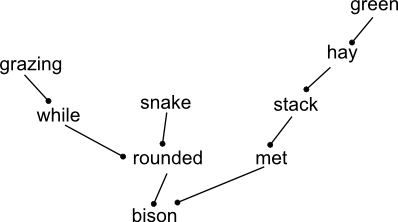
\includegraphics[scale=0.75]{ivans-bison-example.png}
\end{figure}
Notice that the links in the graph are directed, as the application operator is non-commutative, ie,
$$a \circ b \neq b \circ a .$$